\documentclass[11pt,a4paper]{article}
\usepackage[hyperref]{acl2018}

\usepackage{newtxtext}
\usepackage[author={Lyndon}]{pdfcomment}





\usepackage{url}
\usepackage[subtle]{savetrees}

%%%%%%%%%%%
%Graphics
\usepackage{graphicx}
\usepackage{tikz}
\usetikzlibrary{positioning,arrows,shapes,fit,  shapes.geometric}
\tikzset{
	every picture/.style={/utils/exec={\sffamily}},
	every matrix/.style={ampersand replacement=\&, rounded corners=10pt},
	every node/.style = {font=\small, inner sep = 3},
	>=latex,
	every text node part/.style={align=center}, auto,node distance=2.4, ->,
	every edge/.append style={every node/.style={font=\footnotesize}}
}
\usepackage[subpreambles=false]{standalone}

%%%%%%%%%%%
%  Tables
\usepackage{booktabs}
\usepackage{pgfplotstable}
\pgfplotsset{compat=1.14}



\pgfplotstableset{col sep=comma, header=has colnames,
%	numcol/.style={},
	string replace={"}{},
	numeric type, precision=3, fixed zerofill=true,
	%			bf content/.style={postproc cell content/.style={@cell content/.add={1\textbf{##1}}}},
	stringcol/.style={string type, column type={r}},
	%
	columns/Train Set/.style={stringcol},
	columns/Test Set/.style={stringcol},
	columns/Dataset/.style={stringcol},
	columns/Method/.style={stringcol},
	%
	every head row/.style={after row = {\toprule}}
}


%%%%%%%%%%%%%%%%%%%
% Math 

\usepackage{amssymb}
\usepackage{amsmath}
\usepackage{mathtools}
\DeclareMathOperator*{\argmin}{arg\,min}
\DeclareMathOperator*{\argmax}{arg\,max}

\newcommand{\compactmath}[1]{\noindent\resizebox{\columnwidth}{!}{$#1$}}
%%%%%%%%%%%%%%%%%%%%%%%%
\usepackage{cleveref}

%%%%%%%%%%%%%%%%%%%%%%%%%%%%%%%%%%%%
\usepackage{natbib}
\bibliographystyle{apalike}

\newcommand{\parencite}{\citep}
\newcommand{\textcite}{\cite}


%opening
\title{NovelPerspective}
%\author{Lyndon White \\ lyndon.white@research.uwa.edu.au %
%	\and Roberto Togneri \\ roberto.togneri@uwa.edu.au%
%	\and Wei Liu \\ wei.liu@uwa.edu.au %
%	\and Mohammed Bennamoun \\ mohammed.bennamoun@uwa.edu.au %
%}


\begin{document}

\maketitle

\begin{abstract}
We present a proof of concept for a tool to allow consumers to subset ebooks, based on the main character of the section.
Many novels have multiple main characters, and vary with each chapter (or sub-chapter) which character the story is focused on.
A well known example is George R. R. Martin's ``Game of Thrones'' novel, and others from that series.
The NovelPerspective tool detects which character the section is about,
and allows the user to generate a new ebook with only those section.
The detection of main character can be done by many means.
We present two simple baselines, and several machine learning based methods.
\end{abstract}

\section{Introduction}

Many books have multiple main characters, often each character is written from the perspective of a different main character.
Different sections are written from the perspective of different characters.
Generally, these books are written in limited third-person point of view (POV);
that is to say the reader has little or or more knowledge of the situation described than the main character does.
Having a large cast of character, in particular POV characters, is a hallmark of the epic fantasy genre.

We propose a method here to detect the main/POV character for each section of the book.
Detecting the main character is not a difficult task, as the strong baseline result shows.
However to our knowledge there does not exist any current software to do this.
We attribute this lack to it being impractical to physically implement until recent times.
The surge in popularity of ebooks has opened a new niche for consumer discourse processing.
Tools such as the one present here, give the reader new freedoms in controlling how they consume their media.

We focus here on novels written in the limited third-person point of view.
In these stories, the main character is, for our purposes, the point of view (POV) character.
Limited third-person POV is written in the third-person, that is to say the character is referred to by name, but with the observations limited to being from the perspective of that character.
This is in-contrast to the omniscient third-person POV, where events are described by an external narrator.
Limited third-person POV is extremely common in modern fiction.
Well known examples include George R.R. Martin's "A Song of Ice and Fire", 
Robert Jordan's ``Wheel of Time'', Brandon Sanderson's ``Cosmere'' universe, 
Steven Erikson's "Malazan Book of the Fallen".
It preserves the advantages of first person, in allowing the reader to observe inside the head of the character, while also allowing the flexibility to switch to narrate from another character \parencite{booth2010rhetoric}.
This allows for multiple concurrent storylines around different characters.
Our tool helps users un-entwine such storylines, giving the option to process them sequentially.



%Some examples include: 
%Across its 15 books, Robert Jordan's "Wheel of Time" series which has 146 POV characters\footnote{\url{http://wot.wikia.com/w3iki/Statistical_analysis}}). Only about one fifth of the total word count was from the POV of the ``main character''.
%George R.R. Martin's "A Song of Ice and Fire", have over 30 POV characters in the books published so far %\footnote{\url{http://awoiaf.westeros.org/index.php/POV_character}}.

%This is also of interest for works written in omniscient third person point of view, such as J. R. R. Tolkien's ``Lord of the Rings'',
%which also may feature a focus on different main characters however the correct split is much less clear in these cases.



The utility of dividing a book in this way varies with the book in question.
Some books will cease to make sense when the core storyline crosses over different character.
Other novels, particularly the large epic fantasy stories we are primarily considering,
have many parallel story lines focused on the different characters that only rarely intersect.
While we are unable to find formal study on this, 
many readers speak of ``skipping the chapters about the boring characters'',
or ``Only reading the real main character's sections''.
Particularly on a re-read, or after already having consumed the media in some other form such as watching a movie adaptation, or reading a summary.
We note that sub-setting the novel once does not prevent the reader going back and reading the intervening chapters if it ceases to make sense, or from sub-setting again to get the chapters for another character who's path the one they are reading intersects.
We can personally attest for some books reading the chapters one character at a time is indeed possible, and indeed pleasant: the first author having read George R.R. Martin's "A Song of Ice and Fire" series in exactly this fashion.

The primary limitation in segmenting ebooks this way is in classifying the sections as to which character they are from the perspective of.
To solve this, the core of our tool is its character classification systems.
We investigated several options which the main text of this paper will discuss.


\section{Character Classification Systems}
\begin{figure*}
	\resizebox{\textwidth}{!}{
		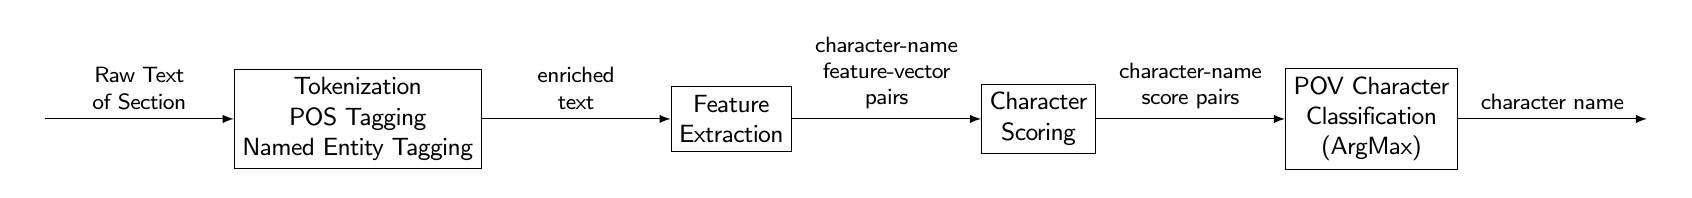
\begin{tikzpicture}		
		\node(start){};
		\node(enrich)[draw, right=of start] {Tokenization\\POS Tagging\\Named Entity Tagging};
		\node(features)[draw, right=of enrich] {Feature\\ Extraction};
		\node(scoring)[draw, right=of features] {Character\\Scoring};				
		\node(classify)[draw, right=of scoring] {POV Character\\ Classification \\(ArgMax)};
		\node(end)[right=of classify] {};
		
		\path (start) edge node[above]{Raw Text \\ of Section}  (enrich);
		\path (enrich) edge node[above]{enriched\\text} (features);
		\path (features) edge node[above]{character-name\\feature-vector\\pairs
		} (scoring);
		\path (scoring) edge node[above]{character-name\\score pairs
	} (classify);
		\path (classify) edge node[above]{character name}  (end);
		\end{tikzpicture}
	}
	\caption{The general structure of the character classification systems. This in turn is the classification step of part of the large stem in \Cref{fig:fullprocess}. \label{fig:classify}}
\end{figure*}
The common structure of all our character classification systems is shown in \Cref{fig:classify}.
First the raw text is enriched with part of speech and named entity targets,
from which features are extracted for each named entity.
Theses are used to score the named entities for the most-likely to be the POV character, and the highest scoring is returned by the system.
The different systems presented modify the the Feature extraction and Character scoring steps.


\subsection{Baseline systems: First and Most Common}
The obvious way to determine the main character of the section is to select the first named entity.
In this system feature extraction and scoring is just to give a score of one to the first named entity found, and zero to the others.
This works well for many examples: ``It was a dark and stormy night. Bill heard a knock at the door.''; however it fails for many others ``'Is that Tom knocking on my door' thought Bill, one storm night.''.
Sometimes a section  may go several paragraphs describing events before it even mentions the character who is perceiving them.
This is a varying element of style.

A more robust method is to use the most commonly named entity.

Here the feature extraction and scoring step scores each named entity proportionate to how often it occurred.
This works well, as once can assume the most commonly named entity is the main character.
However, it is fooled, for example, by book chapters that are about the main character's relationship with a secondary character.
In such cases the secondary character may be mentioned more often.

A better system would combine both the information about when a named entity appeared,
with a how often it occurs, and other information about how that named entity token is being used.
It is not obvious as to how these should be combined to determine which named entity section is about.
We thus attempt to solve it using machine learning, to combine these features to make a classifier.

\subsection{Machine learning systems}
One can see the determination of the main character as a multi-class classification problem.
From the set of all named entities in the section, classify that section as to which one is the main character.
Unlike typical multi-class classification problems
the set of possible classes varies per section being classified.
\pdfcomment{Relate this to named enity detection?}
Further, even the total set of possible named characters, and thus classes, varies from book to book.

An information extraction approach is required which can handle these varying classes.
As such, any machine learning model used can not incorporate knowledge of the classes themselves into it's learned system.

We reconsider the problem as a series of binary predictions.
For each possible character (i.e. each named-entity that occurs), a feature vector is extracted.
This feature vector is the input to a binary classifier, which determines the probability that it represents the main character.
We consider than binary probability as the score for the corresponding character.
We chose the highest scoring character.

It should be noted that the base-line systems, while not using machine learning for the final character classification, they do make extensive use of machine learning based systems during the preprocessing stages (in the same way the machine learning systems to also for preprocessing).
The POS-tagger, and the Named Entity recogniser are based on machine learning.

\subsubsection{Classifier}
XGBoost tree ensemble's are used for the machine learning methods \parencite{chen2016xgboost}.
We use the default hyper-parameters:  100 trees with a max depth of 3,
using the logistic loss function.

During training, from each text in the training dataset,
we generated a training example for every named entity that occurred.
All bar one of these was a negative example.
We then trained it as per normal for a binary classifier, using the logistic loss function.

Theoretically, a better loss function would be a variation on the multi-class hinge-loss \parencite{dogan2016multiclassSVM}, where the objective would be for the true named entity to score higher than any of the other named entities extracted from the same text.



\subsubsection{Feature Extraction}
For the models we investigated several feature sets.
XGBoost is based on decision trees with limited depth.
It thus performs implicit pruning, so we are not concerned with redundant or useless features.
As such we use large numbers of features, many of which are not actually used in the trained model, as discussed in \Cref{sec:featureweights}.


We define the  ``Classical Features-Set'' using features that are well established in NLP related tasks.
We start with the features from the Baseline systems.
The position in the text that the named Entity first occurs, and for symmetry also the last position.
The the number of occurrences, as well as the rank of that score compared to the other named entity in this text.
This occurrence rank is the only feature which gives direct reference to the other possibly labels.
It would be possible to create more rank based-features for the other features.
The other features are based on frequency of each POS tag of the immediately adjacent words.
We theorised that this POS information would be informative, as the it seemed reasonable that the POV character would be described as doing more things, so co-occurring with verbs seemed useful.
This give 100 base features.
To allow for text length invariance we also provide each as a percentage its maximum possible value, For a total of 200 features.

We define a ``Word Embedding Feature-Set'' using FastText word vectors \parencite{bojanowski2016enriching}.
We concatenate the word embedding for the a 5 word window to either size of the named entity;
and take the element-wise mean of this concentrated vector over all occurrences of the named entity.
Such averages of word embeddings have been shown to be a rich and useful feature in many tasks \cite{White2015SentVecMeaning,mikolovSkip}.





\section{Experimental Setup}\label{sec:experimental-setup}
\subsection{Datasets}
We make uses of three series of books selected from our own personal collections.
The first four books of George R. R. Martin's ``A Song of Ice and Fire'' series (hereafter referred to as ASOIAF);
the two books of  Leigh Bardugo's ``Six of Crows'' duology (hereafter referred to as SOC);
and the first three books of Brandon Sanderson's ``Stormlight Archive'' (hereafter referred to as SA).


The requirements of the books to use in the training and evaluation of the NovelPerspective system is that they provide ground truth for the section's POV  character.
ASOIAF and SOC do so in the chapter names.
SA indicates using an chapter image corresponding to the main character.
However, each chapter of SA has sections which feature different POV characters -- many of which do not features as ``main POV'' characters at all.
Thus the ground truth of SA is much weaker.
Better would be to have the sub-chapter sections individually labelled.

We do not have any datasets with labelled sub-chapter sections,
though the tool does support such works.


\begin{table}
	\begin{tabular}{rcc}
		Dataset & Chapters & POV Characters\\
		\toprule
		ASOIAF  & 256	&	15\\
		SOC		& 91	&	9\\
		SA		& 275	&	6
	\end{tabular}
	\caption{Dataset key features. \label{tbl:datasets}}
\end{table}

The total counts of chapters and characters in the datasets, after preprocessing, is shown in \Cref{tbl:datasets}.
Preprocessing consisted of  discarding chapters for which the POV character was not identifies (e.g. prologues); and of removing the character names from the chapter titles as required.

\subsection{Evaluation Details}
In the evaluation, the systems are given the body text and asked to predict the character names.
To mimic the human users ability to select multiple aliases of a character, before final classification the scores of character's nicknames are merged.
For example merging \texttt{Ned} into \texttt{Eddard}.

\subsection{Evaluation Metrics}
We report overall accuracy, and the micro-averaged precision, recall and F1-score \parencite{sokolova2009systematica}.
Note that this means the overall accuracy is the same as the recall.
\pdfcomment{I am  uncertain about the correct metrics to use}.

In the case of the cross-validation results, we report the mean results over 10 random folds, using the same 10 folds for each model being evaluated.

\subsection{Implementation}
The full implementation is available at \url{https://github.com/oxinabox/NovelPerspective/}

The text is preprocessed using NLTK \parencite{NLTK} to added features.
The text is first tokenised, part of speech (POS) tagged , and finally named entity chunked (binary), using NLTK's default methods.
That is the Punkt sentence tokenizer \parencite{kiss2006unsupervised}, regex based improved TreeBank word tokenizer, Greedy Averaged Perceptron POS tagger, and the Max Entropy Named Entity Chunker.
The use of a binary, rather than a multi-class named entity chunker is significant.
Because fantasy novels often use ``exotic'' names for characters, we found that it often  fooled the multi-class named entity recogniser, into thinking characters were organisations or places rather than people.
Note that this is particularly disadvantageous to the First Mentioned Named Entity Baseline, as any kind of named entity will steal the place.
Never-the-less, it is required to ensure that all character names are a possibility to be selected.

Scikit-Learn is used to calculate the evaluation metrics and to orchestrate the cross-validation tests \parencite{scikit-learn}.


\section{Results and Discussion}\label{sec:results-and-discussion}

\subsection{Main results}

\begin{table*}
	\begin{adjustbox}{max width=\textwidth}
		\pgfplotstabletypeset[]{results/maineval.csv}
	\end{adjustbox}
	
	\caption{} \label{tbl:resmain}
\end{table*}

The results of all the methods on both datasets are shown in \Cref{tbl:resmain}.
This includes the two baseline methods, and the machine learning methods with the different feature sets.
The machine learning methods are each train on the dataset which they are not tested on.
As expected the First Mentioned baseline is very weak.

The Most Commonly Mentioned baseline is much stronger.
It marginally outperforms the ML system using Classical Features on the ASIAF dataset.
However, it performs much more poorly on the SOC dataset, 84\% vs 91\% for the Classical Features ML system.
The difference in the Most Commonly Mentioned baseline can be attributed to the difference in writing styles between the novels, how often other characters are being described from the point of view of the (so called) main character.

The Word Embedding model performs generally worse than the classical features model.
This is actually a surprising good result.
The word embedding model contains no features about how frequent the named entity occurs.
Only the average of the word embeddings for its context.
Yet it is still able to generally perform the task.
This suggests that word vector 
\pdfcomment{IDK compare to work embedding feature on cross validation.}

The hybrid results, including both word embedding features, and classical features perform identically to the Classical Features system.
This can be attributed to during training, the word embedding features being found to be less useful, and thus not used in any of the trees.

The weak ground truth of SA can be seen is the relatively poor performance of the ML systems trained on SA, compared to the other ML systems.
\pdfcomment{See if this can be attributed to it learning to only trust most common features,  due to the decreased usefulness of other features as they are actually right for subsets of the text that are mis-labelled}



\subsection{Cross Validation Results}

\begin{table*}
	\begin{adjustbox}{max width=\textwidth}
		\pgfplotstabletypeset[]{results/crosseval.csv}
	\end{adjustbox}
	
	\caption{10 fold cross-validation results. The ML systems are trained and tested on distinct slices of the same dataset. \label{tbl:rescross}}
\end{table*}

To determine the effect of author/book style on the performance of the systems,
we also evaluated them using 10 fold cross validation.
By training and testing on different chapters from within the same book we control for variations in the writing style.
The results are shown in  \Cref{tbl:rescross}.
It can be seen that they are indeed significantly better for the classical features system than the results in \Cref{tbl:resmain} where the systems trained on different books.
With the SOC result being a perfect score
This suggests that indeed the features that indicate a point of view character in one book, do not perfectly transfer to another; but that they are reasonably consistent within a single book.





\subsection{Feature Weights}\label{sec:featureweights}
From a model trained on the full combined dataset,
we can extract the feature weights.





\section{Demonstration}

\begin{figure*}
	\resizebox{\textwidth}{!}{
		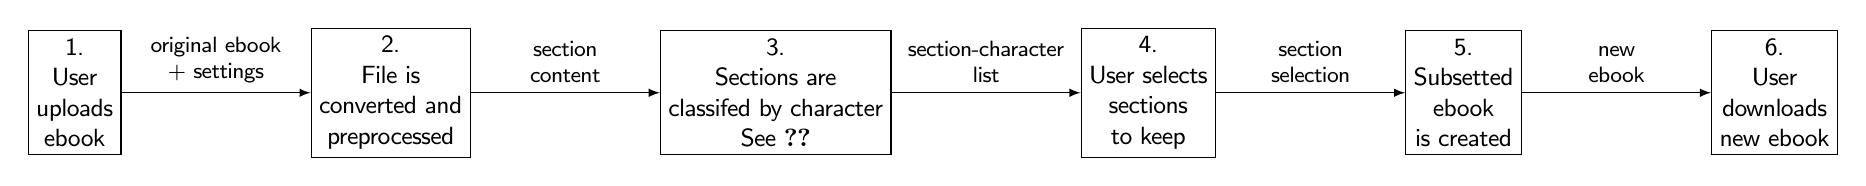
\begin{tikzpicture}		
		\node(start)[draw] {1.\\User\\ uploads\\ ebook};
		\node(convert)[draw, right=of start] {2.\\ File is\\ converted and \\preprocessed};
		\node(classify)[draw, right=of convert] {3.\\Sections are \\ classifed by character\\ See \Cref{fig:classify}};
		\node(select)[draw, right=of classify] {4.\\User selects\\ sections\\ to keep};
		\node(create)[draw, right=of select] {5.\\Subsetted\\ ebook\\ is created};
		\node(download)[draw, right=of create] {6.\\User \\downloads \\ new ebook};
		
		\path (start) edge[below] node[above]{original ebook \\ + settings}  (convert);
		\path (convert) edge[below] node[above]{section\\ content} (classify);
		\path (classify) edge[below] node[above]{section-character\\list} (select);
		\path (select) edge[below] node[above]{section\\selection}  (create);
		\path (create) edge[below] node[above]{new \\ ebook}  (download);	
		\end{tikzpicture}
	}
	\caption{The full process of the using NovelPerspective. Note that step 5 uses the original ebook to subset. \label{fig:fullprocess}
	}
\end{figure*}

An online demonstration is available at \url{http://white.ucc.asn.au/tools/np}.
This is a web-app, made using the CherryPy framework\footnote{\url{http://cherrypy.org/}}.
This allows the user to apply any of the model discussed to their own novels.
With the exclusion of the word embedding based models, as while interesting, these were less performant and much more demanding on computational resources.


The users uploads an ebook, and selects one of the character detection systems we have discussed above.
The users is then presented with a page displaying a list of sections,
with the predicted main character in the left, and an excerpt from the beginning of the section on the right.
To avoid the user having to wait while the whole book is processed this list is dynamically loaded as it is computed.
We find that the majority of the time is spend on running the preprocessing to annotate the data before the classification.

The user can select sections to keep.
This is done via check-boxes to the right of each author
The user can input a regular expression for a character name to have the corresponding check-boxes marked.
This uses the character name as predicted by the model.
As none of the models is perfect, some mistakes are likely to be mode.
The user can then manually correct the selection using the check-boxes before downloading the book.




\section{Conclusion}\label{sec:conclusion}
We have presented a tool to allow consumers to restructure their ebooks around the characters they find most interesting.
The system must discover the named entities present in each section of the book,
and then classify the section as to which character is the Point of View character.
For named entity detection we make use of standard tools.
The classification is non-trivial.
In its design we implemented several systems.
Simply selecting the most commonly named character proved very successful as a baseline approach.
It is outperformed by a machine learning based classifier using classical features: primarily occurrence counts of the named entity, and of the different parts of speech that occur adjacent to it.
While none of the classifiers are perfect,
they achieve high enough accuracy to be useful.

The results are presented to the user via a web-interface.
The user can use the results to select the chapters from the point of view of the character/s they are most interested in;
and correct any errors the system has made.
The user can then download the selected subset of their book.


Further tools along these lines have potential as writing aids for authors.
To allow them to assess how much ``screentime'' is being given to each character of their work in progress novels.
With additional discourse processing, it would be possible to display other useful analytics, such as how often characters occur in the same scenes.

Another application of related work would be the automatic indexing of texts, by adding features such as the main character name, the perspective, etc.
This could be applied to resources such as Wikisource, or Project Gutenberg;
which have texts, but not annotations such as these.




\clearpage
\bibliography{master}
\end{document}
